\chapter{Понятие нейронных сетей, их классификация, основные области применения}
Началом понятия нейронной сети послужила биологическая модель нейрона человеческого мозга.
Уорреном МакКаллокм (Warren McCulloch) и Уолтер Питтс (Walter Pitts) в 1943 году предложили
модель искусственного нейрона, которая получила название перцептрон. Перцептрон принимал на вход $n$ бинарных величин $x_1, \dots x_n$,
которые учитываются с весами $w_1, \dots, w_n$. На основе значения, полученного сумматором $\sum_{i=1}^n x_i w_i$, функция активации
$\varphi$ формирует выходное значение $a$, которое определяется по формуле:
\begin{equation}
    a = \varphi \left( \sum\limits_{i=1}^n x_i w_i \right).
\end{equation}

\begin{figure}[H]
	\center{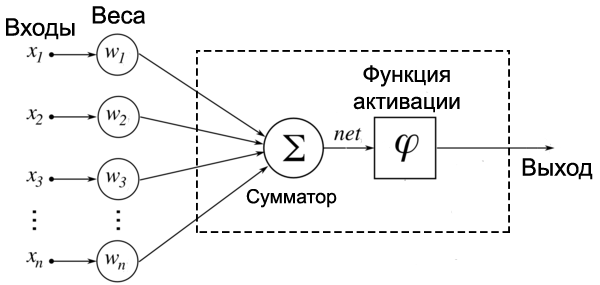
\includegraphics[width=0.7\linewidth]{img/perceptron.png}}
	\caption{Перцептрон}
\end{figure}

Упомянутые ученые также предложили способ объединения искусственных нейронов в сети, называемые нейронными сетями.
Нейроны, находящиеся на одном уровне обработки входных данных, объединялись в слои.
Слой, который принимает сигналы из внешнего мира, называется входным. Слой, который выдает сигналы во внешний мир, —
выходным. Остальные слои называются скрытыми \cite{sozykin}.

Процесс подбора весов называется процессом обучения нейросети.
Обучение происходит на уже имеющемся наборе входных данных и
решений: веса нейросети подбираются так, чтобы в среднем для всей
обучающей выборки ошибка в выходных данных и действительного
решения была минимальна.

Для решения задачи необходимо выбрать определенный набор
нейронов и правильно их соединить. Рабочие модели нейросетей
насчитывают от сотен тысяч до десятков и сотен миллионов нейронов.
Однако отдельные нейроны не используются в составлении нейросетей изза сложности практических задач. Вместо этого используют специальные
наборы с заранее известной структурой. Их называют слоями, а из них в
свою очередь составляются сложные большие нейронные сети, пригодные
для решения задач. Общий вид, или структура, нейросети со всеми слоями,
функциями активации, регуляризации, входными и выходными нейронами
называется архитектурой нейросети \cite{cyber_alex}.

Нейронные сети можно классифицировать в зависимости от различных качеств.
1. По характеру обучения

С учителем, когда известно выходное пространство решений нейронной сети, а также предполагается, что имеются входные сигналы и
эталонные реакции на них. В процессе обучения происходит целенаправленная модификация синаптических связей нейронной сети (NN)
для достижения наилучшего соответствия между реальными выходными значениями сети Y и их эталонными значениями е

Без учителя. В этом случае нейронная сеть формирует выходное
пространство решений только на основе входных воздействий. Такие
сети называются самоорганизующимися

Подкрепляющее обучение (reinforcement learning). Происходит на основе сигнала подкрепления r от внешней среды.

Рекуррентные нейронные сети -- подкласс нейронных сетей с обратными связями, которые
используют предыдущие состояния сети для вычисления текущего. Сеть строится из узлов, каждый
из которых соединѐн со всеми другими узлами. У каждого нейрона порог активации меняется со
временем и является вещественным числом \cite{bguir_rnn}. 
\begin{figure}[H]
	\center{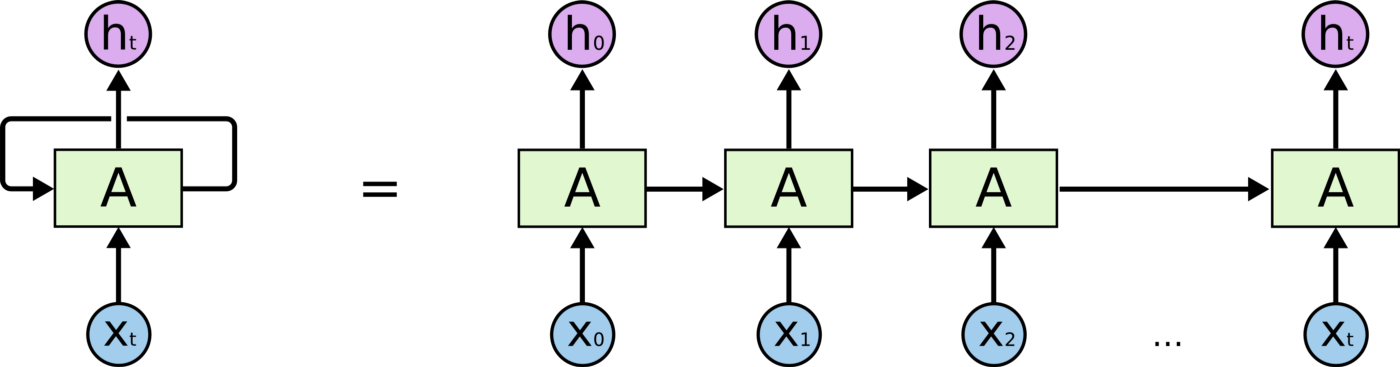
\includegraphics[width=0.7\linewidth]{img/rnn.png}}
	\caption{Иллюстрация работы рекуррентной нейронной сети}
\end{figure}

Автоэнкодерные сети -- подкласс нейронных сетей, для которых характерно наличие сжимающего слоя (энкодера) и восстанавлювающего словя (декодeра).
В процессе вычислений размерность входных данных данных понижается, над которыми далее могут производиться дополнительные преобразования, 
после чего размерность сжатых данных (латентного вектора) повышается \cite{vae}.
\begin{figure}[H]
	\center{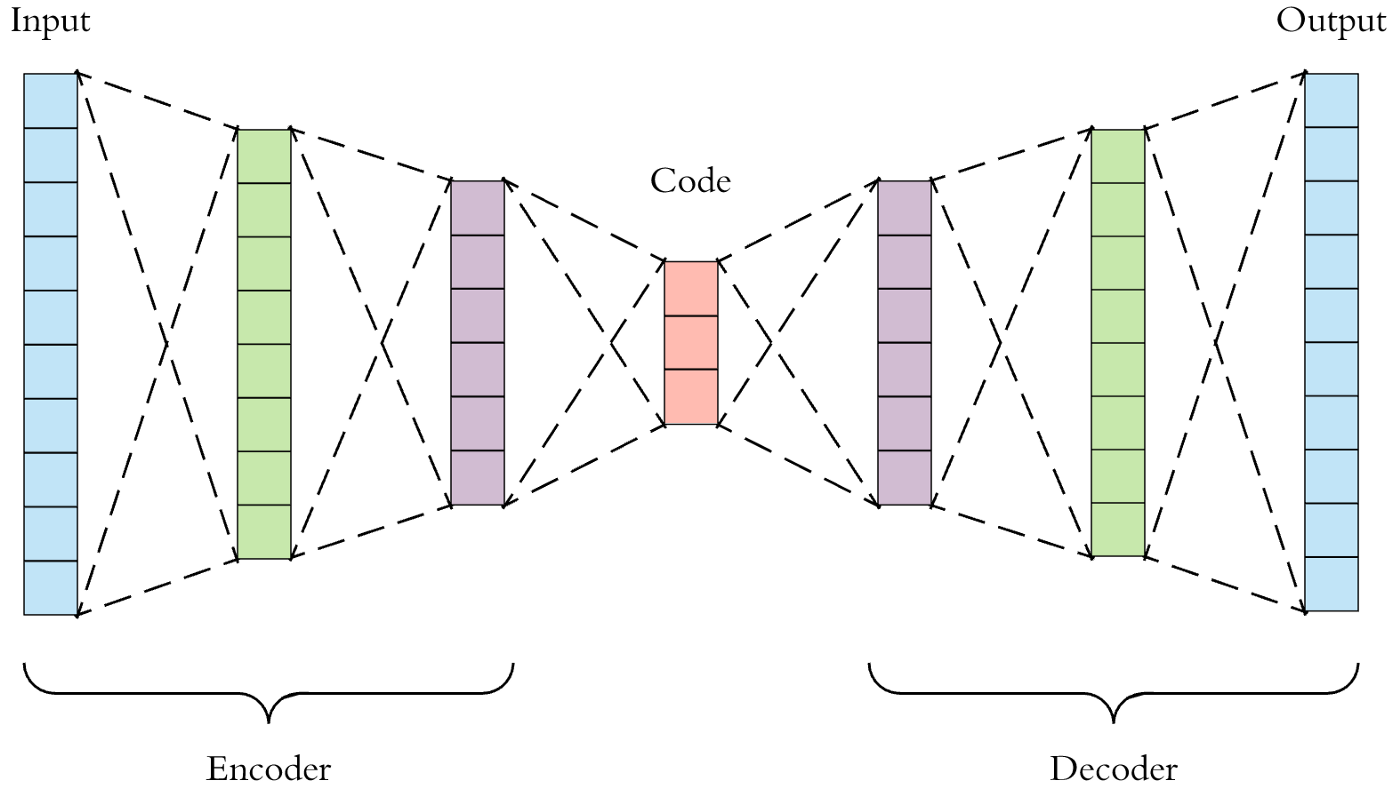
\includegraphics[width=0.7\linewidth]{img/autoencoder.png}}
	\caption{Иллюстрация работы автоэнкодера}
\end{figure}

Автоэнкодерные нейронные сети применяются для выделения наиболее важных информативных признаков 
(feature extraction) во входном пространстве образов, сжатия информации, очистки
данных от шумов, визуализации и классификации данных \cite{bgu_krasn}.

Самоорганизующиеся нейронные сети (self-organising neural networks)
характеризуются обучением без учителя, в результате которого проис-
ходит адаптация сети к решаемой задаче . Их разработал в 80-е гг. XX в.
финский ученый Т. Кохонен (T. Kohonen). Нейронные сети
Кохонена осуществляют топологическое упорядочивание входного
пространства образов, поступающих на сеть. Они широко применяются
в задачах распознавания и визуализации образов, оптимизации и
управления . В данной главе рассматривается архитектура, обучение и
функционирование самоорганизующихся нейронных сетей. Приводится алгоритм решения задачи коммивояжера с использованием сети Кохонена.

\chapter{Основные методы анализа аудиоданных. Анализ аудиоданных при помощи нейросетевых методов}
Аудиоданные многомерны, содержат информацию о частотах закодированного звука с 
определенной периодичностью. 
Для анализа аудиоданных из них извлекают характеристики, характеризующие данные с той или иной стороны.
Примером таких характеристик служат мел-кепстральные коэффициенты (Mel-frequency cepstral coefficients) -- MFCC,
спектральные плотности мощности сигнала в каждый момент времени, 
спектральные полосы, хроматограммы по форме сигнала или по спектрограмме мощности и т.д. \cite{mus_zhao}.
Спектральная плотность мощности $S(\omega)$ сигнала $x(t)$ на промежутке времени $\left[-\frac{T}{2},\frac{T}{2}\right]$ расчитывается как:
\begin{equation}
	S(\omega) = \lim_{T->+\infty} \frac{\left|F_T(\omega)\right|^2}{T},
\end{equation}
где
\begin{equation}
	F_{T}(\omega )={\frac {1}{\sqrt {2\pi }}}\int \limits _{-T/2}^{T/2}x(t)e^{-i\omega t} dt
\end{equation}
-- преобразование Фурье	от $x(t)$ \cite{otnes}.
Зависимость спектральной плотности мощности сигнала от времени характеризуют через изображения -- спектрограммы.
Наиболее распространенным представлением спектрограммы является двумерная диаграмма: на горизонтальной оси представлено время, 
по вертикальной оси — частота; третье измерение с указанием амплитуды на определенной частоте в конкретный момент времени представлено 
интенсивностью или цветом каждой точки изображения.

\begin{figure}[H]
	\center{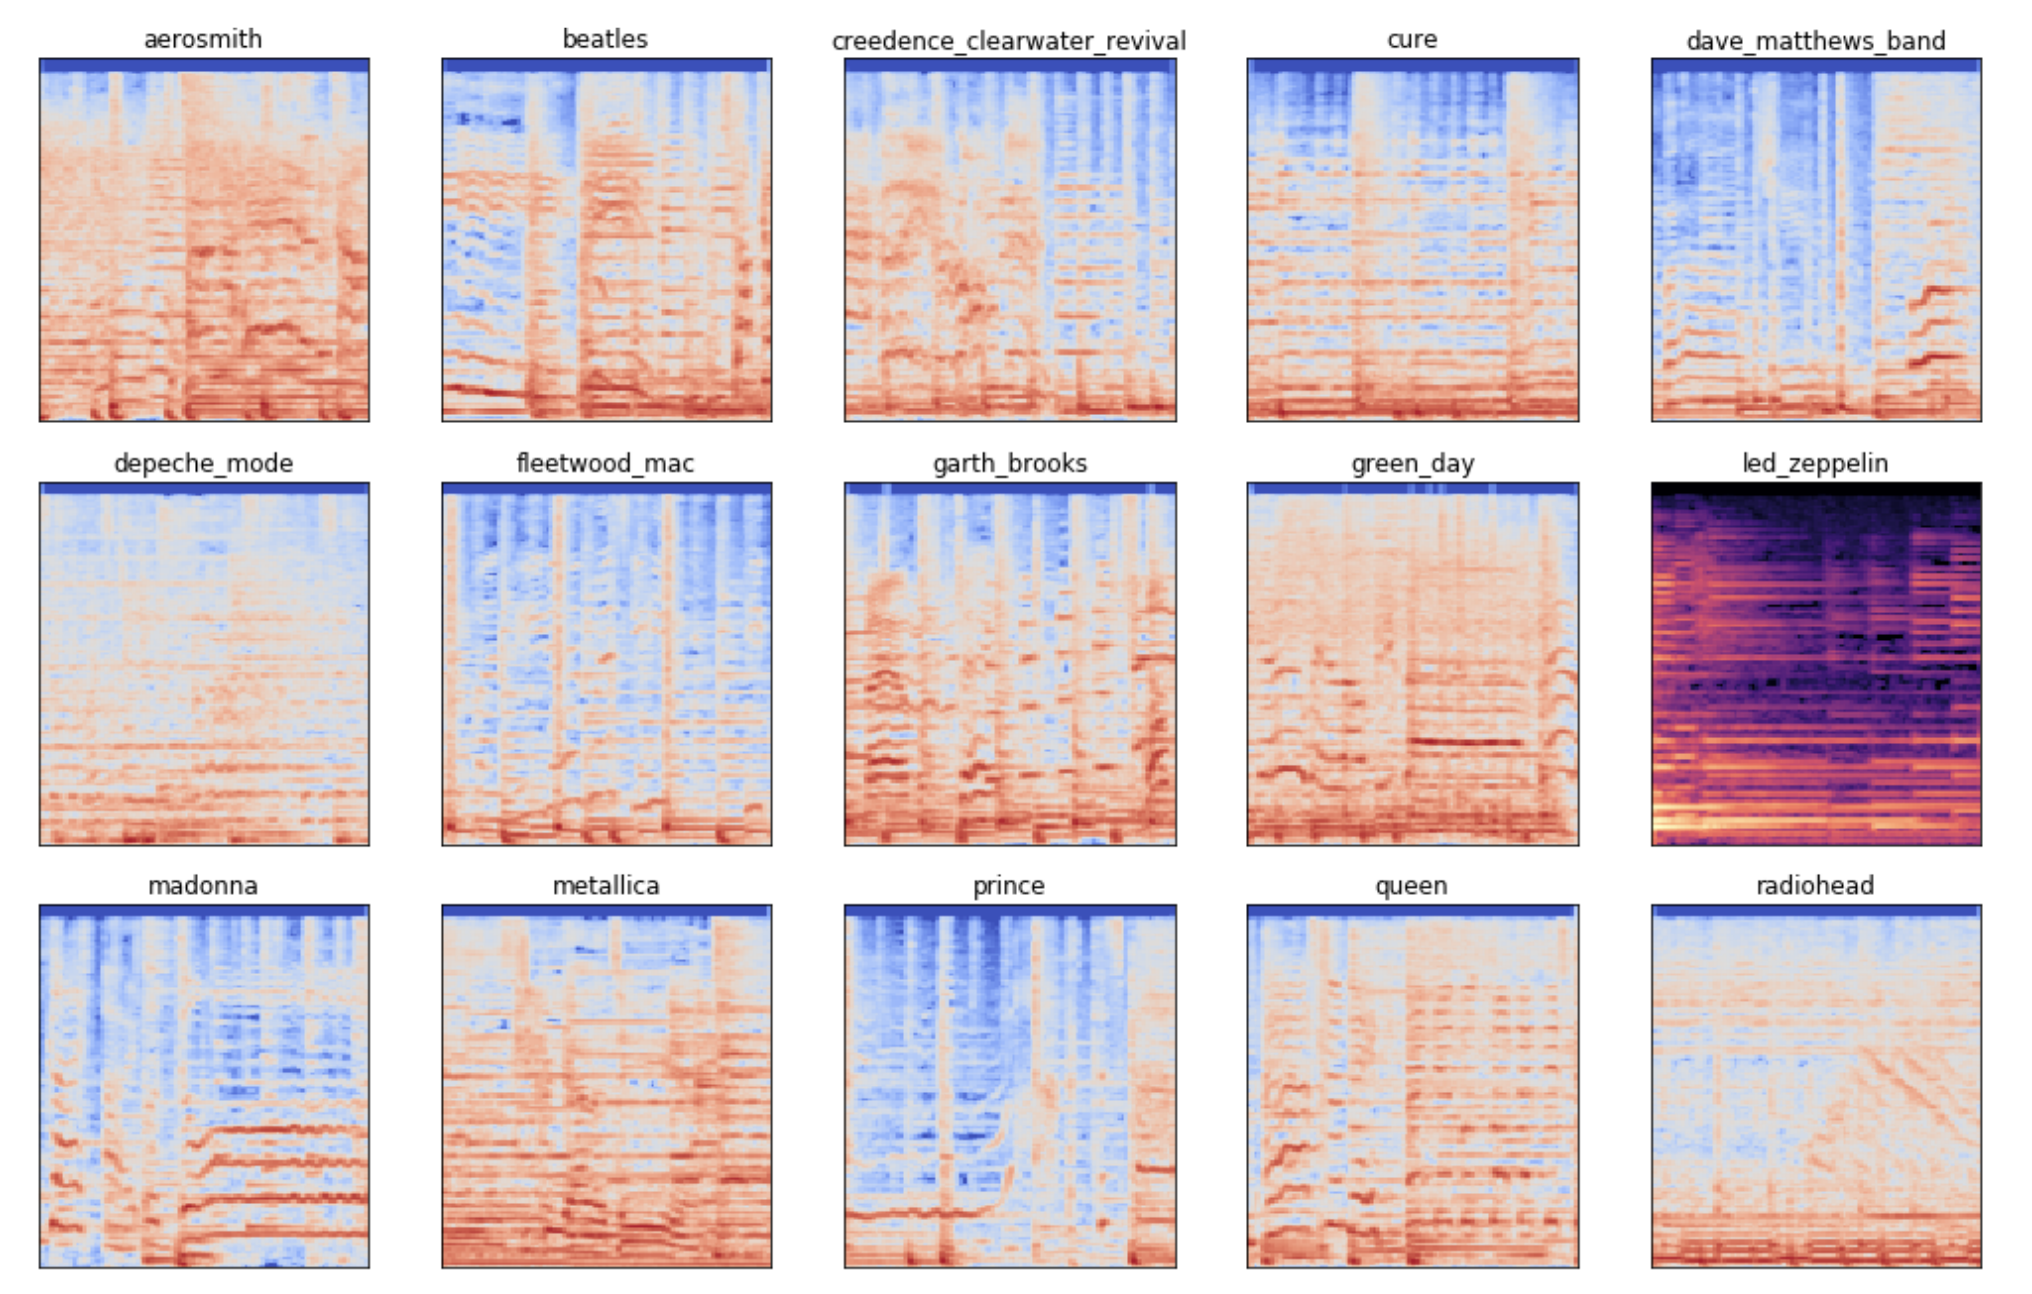
\includegraphics[width=0.7\linewidth]{img/mel.png}}
	\caption{Примеры визуализации спектрограмм композиций популярных исполнителей}
\end{figure}

Возможность представить основные характеристики аудиоданных в виде изображения позволяет применить существующие практики
нейросетевого анализа изображений для анализа и классификации аудиозаписей \cite{cyber_alex}.

\chapter{Особенности подготовки аудиоданных}


\chapter{Кластеризация и классификация аудиоданных при помощи нейронных сетей}
\chapter{Сравнение полученных результатов с априорной классификацией}
\chapter{Общие результаты и выводы}